\newpage
\begin{abox}
	Practise Set-1 \ Solutions
\end{abox}
\begin{enumerate}[label=\color{ocre}\textbf{\arabic*.}]
	\item Consider two point charges $q$ and $\lambda q$ located at the points, $x=a$ and $x=\mu a$,
	respectively. Assuming that the sum of the two charges is constant, what is the value of
	$\lambda$ for which the magnitude of the electrostatic force is maximum?
	{\exyear{JEST 2015}}
	\begin{tasks}(4)
		\task[\textbf{A.}]  $\mu$
		\task[\textbf{B.}]1
		\task[\textbf{C.}]$\frac{1}{\mu}$
		\task[\textbf{D.}] $1+\mu$
	\end{tasks}
	\begin{answer}
		\begin{align*}
		F&=\frac{1}{4 \pi \varepsilon_{0}} \frac{(\lambda q \times q)}{(\mu a-a)^{2}}\\&=\frac{1}{4 \pi \varepsilon_{0}} \frac{\lambda q^{2}}{a^{2}(\mu-1)^{2}}\\&=\frac{1}{4 \pi \varepsilon_{0} a^{2}(\mu-1)^{2}} \frac{\lambda c^{2}}{(1+\lambda)^{2}} \quad \because q+\lambda q\\&=c \\
		\text { For maximum } F, \frac{d F}{d \lambda}=0 \\0&= \frac{1}{4 \pi \varepsilon_{0} a^{2}(\mu-1)^{2}}\left[\frac{(1+\lambda)^{2} c^{2}-\lambda c^{2} \times 2(1+\lambda)}{(1+\lambda)^{4}}\right] \\
		\Rightarrow(1+\lambda)^{2} c^{2}=\lambda c^{2} \times 2(1+\lambda) \Rightarrow 1+\lambda\\&=2 \lambda \\\Rightarrow \lambda&=1
		\end{align*}
		Correct option is (B)
	\end{answer}
\item  An electric field in a region is given by $\vec{E}(x, y, z)=a x \hat{i}+c z \hat{j}+6 b y \hat{k} .$ For which values of
$a, b, c$ does this represent an electrostatic field?
{\exyear{JEST 2012}}

\begin{tasks}(4)
\task[\textbf{A.}]$13,1,12$ 
\task[\textbf{B.}]$17,6,1$
\task[\textbf{C.}]$13,1,6$
\task[\textbf{D.}]$45,6,1$
\end{tasks}
\begin{answer}
\begin{align*}
\intertext{ For electrostatic field,} 
\vec{\nabla} \times \vec{E}&=0\\
\vec{\nabla} \times \vec{E}&=\left[\begin{array}{ccc}
\hat{i} & \hat{j} & \hat{k} \\
\frac{\partial}{\partial x} & \frac{\partial}{\partial y} & \frac{\partial}{\partial z} \\
a x & c z & 6 b y
\end{array}\right]=0\\ \Rightarrow \vec{\nabla} \times \vec{E}&=(6 b-c) \hat{i}+\hat{j}[0-0]+\hat{k}[0]=0 \\
\Rightarrow(6 b-c) \hat{i}&=0 \\\Rightarrow c&=6 b
\end{align*}
Correct option is (C)
\end{answer}
% Question related to Image charge. 
%\question A point charge $+q$ is placed at $(0,0, d)$ above a grounded infinite conducting plane
%defined by $z=0$. There are no charges present anywhere else. What is the magnitude of
%electric field at $(0,0,-d)$ ?
%{\exyear{JEST 2012}}
%\begin{tasks}(4)
%\task[\textbf{A.}]  $\frac{q}{8\pi \in_{0} d^{2}}$
%\task[\textbf{B.}] $-\infty$
%\task[\textbf{C.}]0
%\task[\textbf{D.}]$\frac{q}{16 \pi \in_{0} d^{2}}$
%\end{tasks}
%\begin{answer}
%\begin{align*}
%\intertext{ Electric field at $Q$}
%\vec{E}&=\frac{-q}{4 \pi \epsilon_{0}(2 d)^{2}}(\hat{z})\\&=\frac{-q}{16 \pi \in_{0} d^{2}} \hat{z} \\\Rightarrow|E|&=\frac{q}{16 \pi \in_{0} d^{2}}
%\end{align*}
%Correct option is (D)
%\end{answer}
\item The electric fields outside $(r>R)$ and inside $(r<R)$ a solid sphere with a uniform
volume charge density are given by $\vec{E}_{r>R}=\frac{1}{4 \pi \varepsilon_{0}} \frac{q}{r^{2}} \hat{r}$ and $\vec{E}_{r<R}=\frac{1}{4 \pi \varepsilon_{0}} \frac{q}{R^{3}} r \hat{r}$
respectively, while the electric field outside a spherical shell with a uniform surface
charge density is given by $\vec{E}_{r>R}=\frac{1}{4 \pi \varepsilon_{0}} \frac{q}{r^{2}} \hat{r}, q$ being the total charge. The correct ratio of
the electrostatic energies for the second case to the first case is
{\exyear{JEST 2013}}
\begin{tasks}(4)
\task[\textbf{A.}] $1: 3$
\task[\textbf{B.}]$9: 16$
\task[\textbf{C.}]$3: 8$
\task[\textbf{D.}]$5: 6$
\end{tasks}
\begin{answer}
\begin{align*}
\intertext { Electrostatic energy in spherical shell ,}
w_{s p}&=\frac{\epsilon_{0}}{2} \int_{0}^{R}\left|\vec{E}_{1}\right|^{2} 4 \pi r^{2} d r+\frac{\epsilon_{0}}{2} \int_{R}^{\infty}\left|\vec{E}_{2}\right|^{2} 4 \pi r^{2} d r\\
\Rightarrow \frac{\epsilon_{0}}{2} \int_{R}^{\infty} \frac{q^{2}}{\left(4 \pi \in_{0}\right)^{2} r^{4}} 4 \pi r^{2} d r&=\frac{q^{2}}{8 \pi \in_{0}}\left(-\frac{1}{r}\right)_{R}^{\infty}\\&=\frac{q^{2}}{8 \pi \in_{0}} \frac{1}{R}
\intertext{Electrostatic energy in solid sphere,}
w_{s}&=\frac{\epsilon_{0}}{2} \int_{0}^{R}\left|E_{1}\right|^{2} 4 \pi r^{2} d r+\frac{\epsilon_{0}}{2} \int_{R}^{\infty}\left|E_{2}\right|^{2} 4 \pi r^{2} d r\\
\Rightarrow \frac{q^{2}}{8 \pi \in_{0}}& \times \frac{1}{R^{6}}\left[\frac{r^{5}}{5}\right]_{0}^{R}+\frac{q^{2}}{8 \pi \in_{0}}\left[-\frac{1}{r}\right]_{R}^{\infty}\\
w_{s}&=\frac{q^{2}}{5 \times 8 \pi \in_{0}} \cdot \frac{1}{R}+\frac{q^{2}}{8 \pi \in_{0} R}=\frac{6 q^{2}}{40 \pi \in_{0} R}\\
\text { Now }\ \frac{W_{\text {spherical }}}{W_{\text {sphere }}}&=\frac{\frac{q^{2}}{8 \pi \in_{0}R}}{\frac{6 q^{2}}{40 \pi \in_{0} R}}\\&=\frac{5}{6}
\end{align*}
Correct option is (D)
\end{answer}
\item  If $\vec{E}_{1}=x y \hat{i}+2 y z \hat{j}+3 x z \hat{k}$ and $\vec{E}_{2}=y^{2} \hat{i}+\left(2 x y+z^{2}\right) \hat{j}+2 y z \hat{k}$ then
{\exyear{JEST 2013}}
\begin{tasks}(1)
\task[\textbf{A.}]  Both are impossible electrostatic fields.
\task[\textbf{B.}]Both are possible electrostatic fields.
\task[\textbf{C.}]Only $\vec{E}_{1}$ is a possible electrostatic field.
\task[\textbf{D.}]Only $\vec{E}_{2}$ is a possible electrostatic field.
\end{tasks}
\begin{answer}
\begin{align*}
\text { For electrostatic field } \vec{\nabla} \times \vec{E}=0\\
\vec{\nabla} \times \vec{E}_{2}&=\left|\begin{array}{ccc}
\hat{i} & \hat{j} & \hat{k} \\
\frac{\partial}{\partial x} & \frac{\partial}{\partial y} & \frac{\partial}{\partial z} \\
y^{2} & 2 x y+z^{2} & 2 y z
\end{array}\right|=
(2 z-2 z) \hat{i}+0+(2 y-2 y) \hat{z}=0\\
\vec{\nabla} \times \vec{E}_{1}&=\left|\begin{array}{ccc}
\hat{i} & \hat{j} & \hat{k} \\
\frac{\partial}{\partial x} & \frac{\partial}{\partial y} & \frac{\partial}{\partial z} \\
x y & 2 y z & 3 x z
\end{array}\right|=(0-2 y) \hat{i}+0+x \hat{j} \neq 0
\end{align*}
Correct option is (D)
\end{answer}
\item A charge $q$ is placed at the centre of an otherwise neutral dielectric sphere of radius $a$
and relative permittivity $\varepsilon_{r} .$ We denote the expression $q / 4 \pi \varepsilon_{0} r^{2}$ by $E(r)$. Which of the
following statements is false?
{\exyear{JEST 2013}}
\begin{tasks}(1)
\task[\textbf{A.}] The electric field inside the sphere, $r<a$, is given by $E(r) / \varepsilon_{r}$
\task[\textbf{B.}] The field outside the sphere, $r>a$, is given by $E(r)$
\task[\textbf{C.}]The total charge inside a sphere of radius $r>a$ is given by $q$.
\task[\textbf{D.}]The total charge inside a sphere of radius $r<a$ is given by $q$. 
\end{tasks}
\begin{answer}
Correct option is (D)
\end{answer}
\item Two large nonconducting sheets one with a fixed uniform positive charge and another
with a fixed uniform negative charge are placed at a distance of 1 meter from each other.
The magnitude of the surface charge densities are $\sigma_{+}=6.8 \mu \mathrm{C} / \mathrm{m}^{2}$ for the positively
charged sheet and $\sigma_{-}=4.3 \mu \mathrm{C} / \mathrm{m}^{2}$ for the negatively charged sheet. What is the electric
field in the region between the sheets?
{\exyear{JEST 2014}}
\begin{tasks}(4)
\task[\textbf{A.}] $6.30 \times 10^{5} \mathrm{~N} / \mathrm{C}$
\task[\textbf{B.}]$3.84 \times 10^{5} \mathrm{~N} / \mathrm{C}$
\task[\textbf{C.}] $1.40 \times 10^{5} \mathrm{~N} / \mathrm{C}$
\task[\textbf{D.}] $1.16 \times 10^{5} \mathrm{~N} / \mathrm{C}$ 
\end{tasks}
\begin{answer}
\begin{align*}
\text { Electric field between the sheet is }&=\frac{\sigma_{+}}{2 \epsilon_{0}}+\frac{\sigma_{-}}{2 \epsilon_{0}}\\&=\frac{6.8 \times 10^{-6}}{2 \epsilon_{0}}+\frac{4.3 \times 10^{-6}}{2 \epsilon_{0}}\\
\frac{11.2 \times 10^{-6}}{2 \times 8.86 \times 10^{-12}}&=0.626 \times 10^{6} \Rightarrow 6.3 \times 10^{5} \mathrm{~N} / \mathrm{C}
\end{align*}
Correct option is (A)
\end{answer}
\item A circular loop of radius $R$, carries a uniform line charge density $\lambda$. The electric field,
calculated at a distance $z$ directly above the center of the loop, is maximum if $z$ is equal
to,
{\exyear{JEST 2015}}
\begin{tasks}(4)
\task[\textbf{A.}] $\frac{R}{\sqrt{3}}$
\task[\textbf{B.}] $\frac{R}{\sqrt{2}}$
\task[\textbf{C.}]$\frac{R}{2}$
\task[\textbf{D.}]$2 R$ 
\end{tasks}
\begin{answer}
\begin{align*}
E&=\frac{1}{4 \pi \varepsilon_{0}} \frac{(\lambda \times 2 \pi R) z}{\left(R^{2}+z^{2}\right)^{3 / 2}} \\
\text { For maximum } E,\  \frac{d E}{d z}&=0 \\\Rightarrow \frac{\lambda \times 2 \pi R}{4 \pi \varepsilon_{0}}\left[\frac{\left(R^{2}+z^{2}\right)^{3 / 2}-z \times 3 / 2 \sqrt{R^{2}+z^{2}} \times 2 z}{\left(R^{2}+z^{2}\right)^{3}}\right]&=0 \\
\Rightarrow\left(R^{2}+z^{2}\right)^{3 / 2}&=3 z^{2} \sqrt{R^{2}+z^{2}}\\ \Rightarrow R^{2}+z^{2}&=3 z^{2}\\ \Rightarrow R^{2}&=2 z^{2}\\ \Rightarrow z&=\frac{R}{\sqrt{2}}
\end{align*}
Correct option is (B)
\end{answer}
\end{enumerate}
\newpage
\begin{abox}
	Practise Set-2 \ Solutions
\end{abox}
\begin{enumerate}[label=\color{ocre}\textbf{\arabic*.}]
\item Four equal point charges are kept fixed at the four vertices of a square. How many neutral points (i.e. points where the electric field vanishes) will be found inside the square?
{\exyear{NET/JRF(DEC-2011)}}
\begin{tasks}(4)
	\task[\textbf{A.}] 1
	\task[\textbf{B.}] 4
	\task[\textbf{C.}] 5
	\task[\textbf{D.}] 7
\end{tasks}
\begin{answer}
	\begin{align*}
	\intertext{Inside the square, there is only one point where field vanishes It is at the center of the square}
	\end{align*}
	So the correct answer is \textbf{Option (A)}
\end{answer}
\question A static charge distribution gives rise to an electric field of the form $\vec{E}=\alpha\left(1-e^{-r / R}\right) \frac{\hat{r}}{r^{2}}$, where $\alpha$ and $R$ are positive constants. The charge contained within a sphere of radius $R$, centred at the origin is
{\exyear{NET/JRF(DEC-2011)}}
\begin{tasks}(4)
	\task[\textbf{A.}] $\pi \alpha \varepsilon_{0} \frac{e}{R^{2}}$
	\task[\textbf{B.}]  $\pi \alpha \varepsilon_{0} \frac{e^{2}}{R^{2}}$
	\task[\textbf{C.}] $4 \pi \alpha \varepsilon_{0} \frac{R}{e}$
	\task[\textbf{D.}] $\pi \alpha \varepsilon_{0} \frac{R^{2}}{e}$
\end{tasks}
\begin{answer}
	\begin{align*}
	Q_{e n c}&=\varepsilon_{0} \oint \vec{E} \cdot d \vec{a}\\&=\alpha \varepsilon_{0} \int\left(1-e^{-r / R}\right) \frac{\hat{r}}{r^{2}} \cdot\left(r^{2} \sin \theta d \theta d \phi \hat{r}\right)\\&=\alpha \varepsilon_{0} \times \int_{0}^{\pi} \int_{0}^{2 \pi}\left(1-e^{-r / R}\right) \sin \theta d \theta d \phi\\
	\text{at }r&=R, \quad Q_{e n c}=4 \pi \alpha \varepsilon_{0}\left(1-\frac{1}{e}\right).\text{ So none of the options given are correct.}
	\end{align*}
	None of the options given are correct
\end{answer}
	\question Charges $Q, Q$ and $-2 Q$ are placed on the vertices of an equilateral triangle $A B C$ of sides of length $a$, as shown in the figure. The dipole moment of this configuration of charges, irrespective of the choice of origin, is
{\exyear{NET/JRF(JUNE-2012)}}

\begin{figure}[H]
\centering
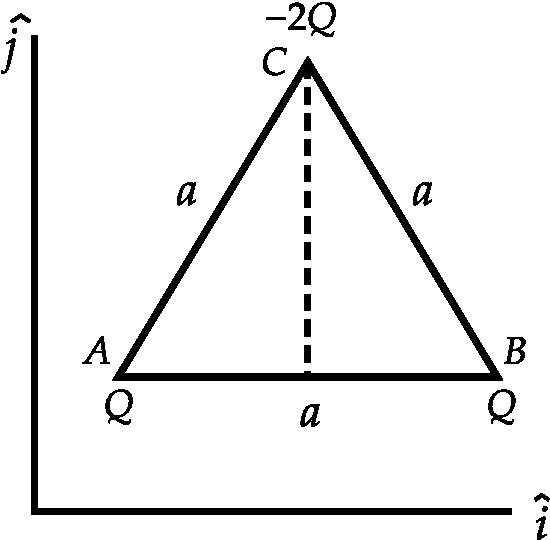
\includegraphics[height=4.5cm,width=4cm]{diagram-20211011(16)-crop}
\caption{}
\label{}
\end{figure}
\begin{tasks}(4)
\task[\textbf{A.}] $+2 a Q \hat{i}$
\task[\textbf{B.}] $+\sqrt{3} a Q \hat{j}$
\task[\textbf{C.}] $-\sqrt{3} a Q \hat{j}$
\task[\textbf{D.}] 0
\end{tasks}
\begin{answer}
\begin{align*}
\intertext{Let coordinates of $A$ is $(l, m)$, then}
\vec{p}&=q_{i} \vec{r}_{i}=Q[l \hat{i}+m \hat{j}]+Q[(l+a) \hat{i}+m \hat{j}]-2 Q\left[\left(l+\frac{a}{2}\right) \hat{i}+\left(m+\frac{\sqrt{3} a}{2}\right) \hat{j}\right]\\
\vec{p}&=Q[l\hat{i}+m \hat{j}]+Q[(l+a) \hat{i}+m \hat{j}]-Q[(2 l+a) \hat{i}+(2 m+\sqrt{3} a) \hat{j}\rfloor \\ \vec{p}&=-\sqrt{3} a Q \hat{j}
\end{align*}
So the correct answer is \textbf{Option (C)}
\end{answer}
\item  Three charges are located on the circumference of a circle of radius $R$ as shown in the figure below. The two charges $Q$ subtend an angle $90^{\circ}$ at the centre of the circle. The charge $q$ is symmetrically placed with respect to the charges $Q$. If the electric field at the centre of the circle is zero, what is the magnitude of $Q$ ?
{\exyear{NET/JRF(DEC-2012)}}

\begin{figure}[H]
\centering
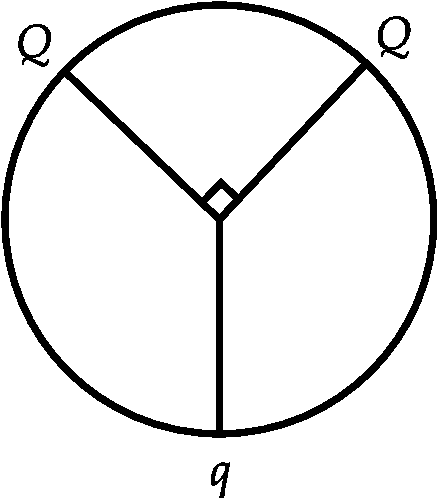
\includegraphics[height=4.5cm,width=4cm]{diagram-20211011(17)-crop}
\end{figure}
\begin{tasks}(4)
\task[\textbf{A.}] $q / \sqrt{2}$
\task[\textbf{B.}] $\sqrt{2} q$
\task[\textbf{C.}] $2 q$
\task[\textbf{D.}] $4 q$
\end{tasks}
\begin{answer}
\begin{align*}
E_{1}&=E_{2}=\frac{1}{4 \pi \varepsilon_{0}} \frac{Q}{R^{2}}\text{ and }E_{3}=\frac{1}{4 \pi \varepsilon_{0}} \frac{q}{R^{2}}\\
\text{Resultant of }E_{1}\text{ and }E_{2}\text{ is }E&=\sqrt{E_{1}^{2}+E_{2}^{2}}=\sqrt{2} E_{1},\\\text{ Thus }E_{3}&=E \\ Q&=\frac{q}{\sqrt{2}}
\end{align*}
So the correct answer is \textbf{Option (A)}
\end{answer}
\item  A point charges $q$ of mass $m$ is kept at a distance $d$ below a grounded infinite conducting sheet which lies in the $x y$ - plane. For what value of $d$ will the charge remains stationary?
{\exyear{NET/JRF(DEC-2012)}}

\begin{tasks}(2)
\task[\textbf{A.}] $q / 4 \sqrt{m g \pi \varepsilon_{0}}$
\task[\textbf{B.}] $q / \sqrt{m g \pi \varepsilon_{0}}$
\task[\textbf{C.}] There is no finite value of $d$
\task[\textbf{D.}]  $\sqrt{m g \pi \varepsilon_{0}} / q$
\end{tasks}
\begin{answer}
There is attractive force between point charge $q$ and grounded conducting sheet that can be calculate from method of images i.e.
\begin{align*}
\frac{1}{4 \pi \varepsilon_{0}} \frac{q^{2}}{(2 d)^{2}}&=m g \\ d&=\frac{q}{4 \sqrt{m g \pi \varepsilon_{0}}}
\end{align*} 
So the correct answer is \textbf{Option (A)}
\end{answer}
\item A solid sphere of radius $R$ has a charge density, given by
$$
\rho(r)=\rho_{0}\left(1-\frac{a r}{R}\right)
$$
where $r$ is the radial coordinate and $\rho_{0}, a$ and $R$ are positive constants. If the magnitude of the electric field at $r=R / 2$ is $1.25$ times that at $r=R$, then the value of $a$ is
{\exyear{NET/JRF(DEC-2014)}}

\begin{tasks}(4)
\task[\textbf{A.}] 2
\task[\textbf{B.}] 1
\task[\textbf{C.}]  $1 / 2$
\task[\textbf{D.}] $1 / 4$
\end{tasks}
\begin{answer}
\begin{align*}
\oint_{S} \vec{E} \cdot d \vec{a}&=\frac{1}{\varepsilon_{0}} Q_{e n c} \Rightarrow|\vec{E}| \times 4 \pi r^{2}=\frac{1}{\varepsilon_{0}} \int_{0}^{r} \rho_{0}\left(1-\frac{a r}{R}\right) 4 \pi r^{2} d r\\
\Rightarrow|\vec{E}| \times 4 \pi r^{2}&=\frac{4 \pi \rho_{0}}{\varepsilon_{0}} \int_{0}^{r}\left(r^{2}-\frac{a r^{3}}{R}\right) d r\\&=\frac{4 \pi \rho_{0}}{\varepsilon_{0}}\left(\frac{r^{3}}{3}-\frac{a r^{4}}{4 R}\right) \Rightarrow|\vec{E}|=\frac{\rho_{0}}{\varepsilon_{0}}\left(\frac{r}{3}-\frac{a r^{2}}{4 R}\right)\\
\because E_{r=R / 2}&=1.25 E_{r=R} \Rightarrow \frac{\rho_{0}}{\varepsilon_{0}}\left(\frac{R / 2}{3}-\frac{a R^{2} / 4}{4 R}\right)=1.25 \frac{\rho_{0}}{\varepsilon_{0}}\left(\frac{R}{3}-\frac{a R^{2}}{4 R}\right)\\
\Rightarrow\left(\frac{1}{6}-\frac{a}{16}\right)&=\frac{5}{4}\left(\frac{1}{3}-\frac{a}{4}\right) \Rightarrow\left(\frac{1}{6}-\frac{a}{16}\right)\\&=\left(\frac{5}{12}-\frac{5 a}{16}\right) \Rightarrow \frac{5 a}{16}-\frac{a}{16}=\frac{5}{12}-\frac{1}{6}\\
\Rightarrow \frac{4 a}{16}&=\frac{5-2}{12} \Rightarrow \frac{a}{4}=\frac{3}{12} \Rightarrow a=1
\end{align*}
So the correct answer is \textbf{Option (B)}
\end{answer}
	\item Consider a charge $Q$ at the origin of 3 - dimensional coordinate system. The flux of the electric field through the curved surface of a cone that has a height $h$ and a circular base of radius $R$ (as shown in the figure) is
{\exyear{NET/JRF(DEC-2015)}}

\begin{figure}[H]
\centering
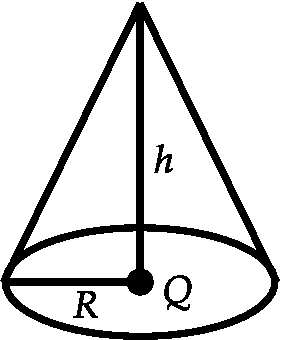
\includegraphics[height=3cm,width=2.5cm]{diagram-20211011(36)-crop}
\end{figure}
\begin{tasks}(4)
\task[\textbf{A.}] $\frac{Q}{\epsilon_{0}}$
\task[\textbf{B.}] $\frac{Q}{2 \epsilon_{0}}$
\task[\textbf{C.}] $\frac{h Q}{R \in_{0}}$
\task[\textbf{D.}] $\frac{Q R}{2 h \in_{0}}$
\end{tasks}
\begin{answer}
So the correct answer is \textbf{Option (B)}
\end{answer}
\item Four equal charges of $+Q$, each are kept at the vertices of a square of side $R$. A particle of mass $m$ and charge $+Q$ is placed in the plane of the square at a short distance $a(\ll R)$ from the centre. If the motion of the particle is confined to the plane, it will undergo small oscillations with an angular frequency
{\exyear{NET/JRF(JUNE-2016)}}

\begin{tasks}(4)
\task[\textbf{A.}] $\sqrt{\frac{Q^{2}}{2 \pi \varepsilon_{0} R^{3} m}}$
\task[\textbf{B.}] $\sqrt{\frac{Q^{2}}{\pi \varepsilon_{0} R^{3} m}}$
\task[\textbf{C.}] $\sqrt{\frac{\sqrt{2} Q^{2}}{\pi \varepsilon_{0} R^{3} m}}$
\task[\textbf{D.}] $\sqrt{\frac{Q^{2}}{4 \pi \varepsilon_{0} R^{3} m}}$
\end{tasks}
\begin{answer}$\left. \right. $
\begin{figure}[H]
	\centering
	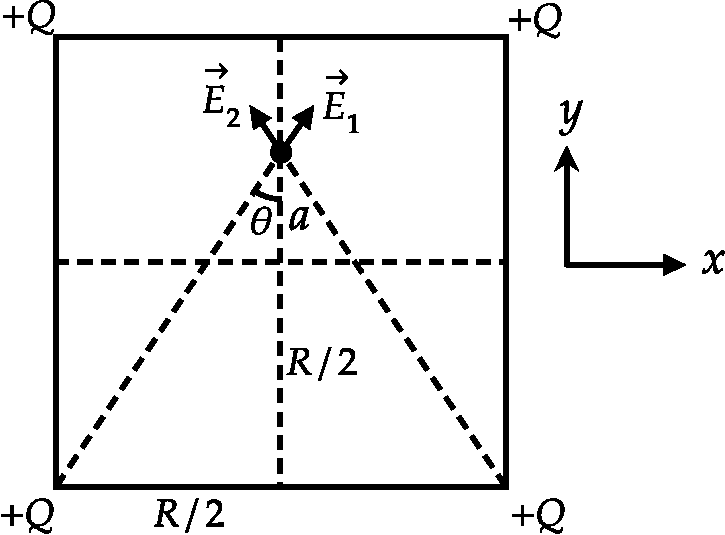
\includegraphics[height=5cm,width=7cm]{diagram-20211011(39)-crop}
\end{figure}
\begin{align*}
E_{1}&=E_{2}=\frac{k Q}{\left[\left(a+\frac{R}{2}\right)^{2}+\frac{R^{2}}{4}\right]}\\
\text{Resultant field }E_{12, y}&=2 E_{1} \cos \theta\\
E_{12, y}&=\frac{2 k Q}{\left[\left(a+\frac{R}{2}\right)^{2}+\frac{R^{2}}{4}\right]^{\frac{3}{2}}}\left(a+\frac{R}{2}\right) \approx \frac{2 k Q}{\left[\frac{R^{2}}{2}\right]^{\frac{3}{2}}}\left(a+\frac{R}{2}\right)\\
E_{12, y}&=\frac{4 \sqrt{2} k Q}{R^{3}}\left(a+\frac{R}{2}\right)\\
\end{align*}
\begin{figure}[H]
	\centering
	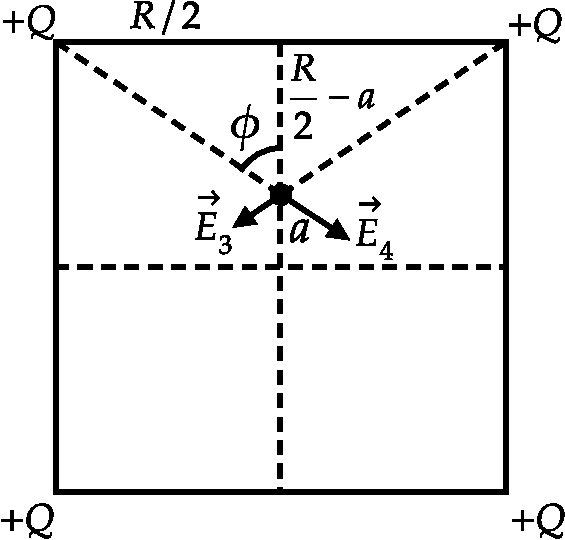
\includegraphics[height=5cm,width=5.5cm]{diagram-20211011(40)-crop}
\end{figure}
\begin{align*}
\text{	Similarly; }E_{3}&=E_{4}=\frac{k Q}{\left[\left(\frac{R}{2}-a\right)^{2}+\frac{R^{2}}{4}\right]}\\
\text{Resultant }E_{34, y}&=2 E_{3} \cos \phi
=\frac{2 k Q}{\left[\left(\frac{R}{2}-a\right)^{2}+\frac{R^{2}}{4}\right]^{\frac{3}{2}}}\left(\frac{R}{2}-a\right)\\
\Rightarrow \quad E_{34, y}&=\frac{4 \sqrt{2} k Q}{R^{3}}\left(\frac{R}{2}-a\right)\\
\text{Resultant }E&=\frac{4 \sqrt{2} k Q}{R^{3}}\left[\left(\frac{R}{2}-a\right)-\left(\frac{R}{2}+a\right)\right]=-\frac{8 \sqrt{2} k Q}{R^{3}} a\\
E&=\frac{-8 \sqrt{2}}{R^{3}} \times \frac{1}{4 \pi \varepsilon_{0}} Q a \\ E&=-\frac{2 \sqrt{2} Q}{\pi \varepsilon_{0} R^{3}} a\\
\Rightarrow \quad F&=Q E=-\frac{2 \sqrt{2} Q^{2}}{\pi \varepsilon_{0} R^{3}} a \\ \omega&=\sqrt{\frac{2 \sqrt{2} Q^{2}}{\pi \varepsilon_{0} m R^{3}}}
\end{align*}
So the correct answer is \textbf{Option (C)}
\end{answer}
\item Consider a sphere $S_{1}$ of radius $R$ which carries a uniform charge of density $\rho$. A smaller sphere $S_{2}$ of radius $a<\frac{R}{2}$ is cut out and removed from it. The centres of the two spheres are separated by the vector $\vec{b}=\frac{\hat{n} R}{2}$, as shown in the figure. The electric field at a point $P$ inside $S_{2}$ is
{\exyear{NET/JRF(JUNE-2016)}}

\begin{figure}[H]
\centering
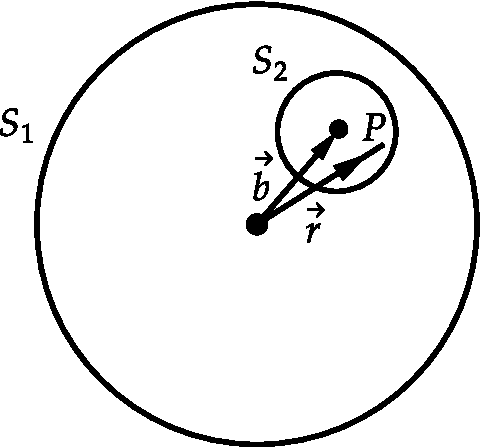
\includegraphics[height=4cm,width=4.2cm]{diagram-20211011(43)-crop}
\end{figure}
\begin{tasks}(4)
\task[\textbf{A.}]$\frac{\rho R}{3 \varepsilon_{0}} \hat{n}$
\task[\textbf{B.}] $\frac{\rho R}{3 \varepsilon_{0} a}(\vec{r}-\hat{n} a)$
\task[\textbf{C.}] $\frac{\rho R}{6 \varepsilon_{0}} \hat{n}$
\task[\textbf{D.}] $\frac{\rho a}{3 \varepsilon_{0} R} \vec{r}$ 
\end{tasks}
\begin{answer}$\left. \right. $
\begin{figure}[H]
	\centering
	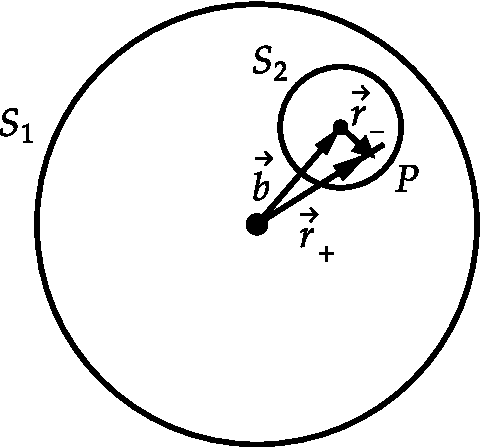
\includegraphics[height=4cm,width=4.2cm]{diagram-20211011(44)-crop}
\end{figure}
\begin{align*}
\text{Electric field at $P$ due to $S_{1}$ is }\vec{E}_{1}&=\frac{\rho}{3 \varepsilon_{0}} \vec{r}_{+}
\intertext{Electric field at $P$ due to $S_{2}$ (assume $\left.-\rho\right)$ is $\vec{E}_{2}=\frac{-\rho}{3 \varepsilon_{0}} \vec{r}_{-}$}
\text{Thus }\vec{E}&=\vec{E}_{1}+\vec{E}_{2}=\frac{\rho}{3 \varepsilon_{0}}\left(\vec{r}_{+}-\vec{r}_{-}\right) ; \\ \because \vec{b}+\vec{r}_{-}&=\vec{r}_{+} \Rightarrow \vec{r}_{+}-\vec{r}=\vec{b}\\
\vec{E}&=\frac{\rho}{3 \varepsilon_{0}} \vec{b}=\frac{\rho R}{6 \varepsilon_{0}} \hat{n}\left(\because \vec{b}=\frac{R}{2} \hat{n}\right)
\end{align*}
So the correct answer is \textbf{Option (C)}
\end{answer}
\item  The charge per unit length of a circular wire of radius $a$ in the $x y$-plane, with its centre at the origin, is $\lambda=\lambda_{0} \cos \theta$, where $\lambda_{0}$ is a constant and the angle $\theta$ is measured from the positive $x$-axis. The electric field at the centre of the circle is
{\exyear{NET/JRF(DEC-2016)}}

\begin{tasks}(4)
\task[\textbf{A.}] $\vec{E}=-\frac{\lambda_{0}}{4 \in_{0} \alpha} \hat{i}$
\task[\textbf{B.}] $\vec{E}=\frac{\lambda_{0}}{4 \in_{0} \alpha} \hat{i}$
\task[\textbf{C.}] $\vec{E}=-\frac{\lambda_{0}}{4 \in_{0} \alpha} \hat{j}$
\task[\textbf{D.}] $\vec{E}=\frac{\lambda_{0}}{4 \pi \in_{0} \alpha} \hat{k}$
\end{tasks}
\begin{answer}$\left. \right. $\\
\begin{figure}[H]
	\centering
	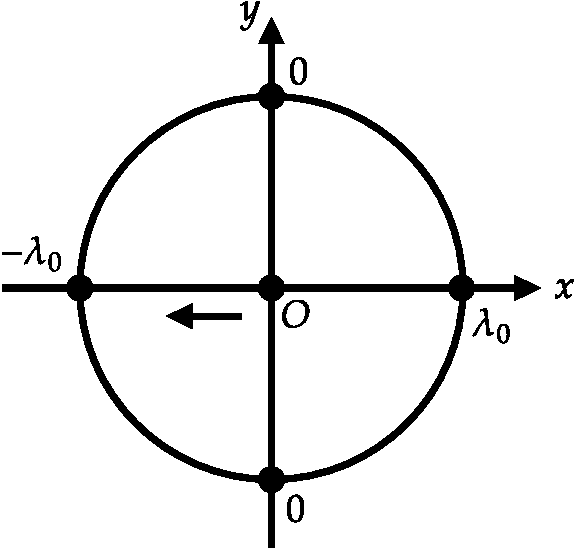
\includegraphics[height=4cm,width=4.1cm]{diagram-20211011(47)-crop}
\end{figure}


Electric field due to a charged element at $P$ is
\begin{align*}
E&=-(d E \cos \theta) \hat{i}-(d E \sin \theta) \hat{j}
\intertext{So, the total electric field at the centre is}
\vec{E} &=-\hat{i} \int d E \cos \theta-\hat{j} \int d E \sin \theta \\
\vec{E} &=-i \int \frac{\lambda d \ell}{4 \pi \varepsilon_{0} a^{2}} \cos \theta-j \int \frac{\lambda d \ell}{4 \pi \varepsilon_{0} a^{2}} \sin \theta \\
&=-\frac{\hat{i} \lambda_{0}}{4 \pi \varepsilon_{0} a^{2}} a \int_{0}^{2 \pi} \cos ^{2} \theta d \theta-\frac{\hat{j} \lambda_{0}}{4 \pi \varepsilon_{0} a^{2}} a \int_{0}^{2 \pi} \cos \theta \sin \theta d \theta \\
&=-\frac{\hat{i} \lambda_{0}}{4 \pi \varepsilon_{0} a} \int_{0}^{2 \pi} \cos ^{2} \theta d \theta=-\hat{i} \frac{\lambda_{0}}{4 \pi \varepsilon_{0} a} \pi=-\frac{\lambda_{0}}{4 \varepsilon_{0} a} i
\end{align*}


At centre $O$, direction of field is $-\hat{x}$.\\
So the correct answer is \textbf{Option (A)}
\end{answer}
\end{enumerate}


